\begin{figure}
  \centering
  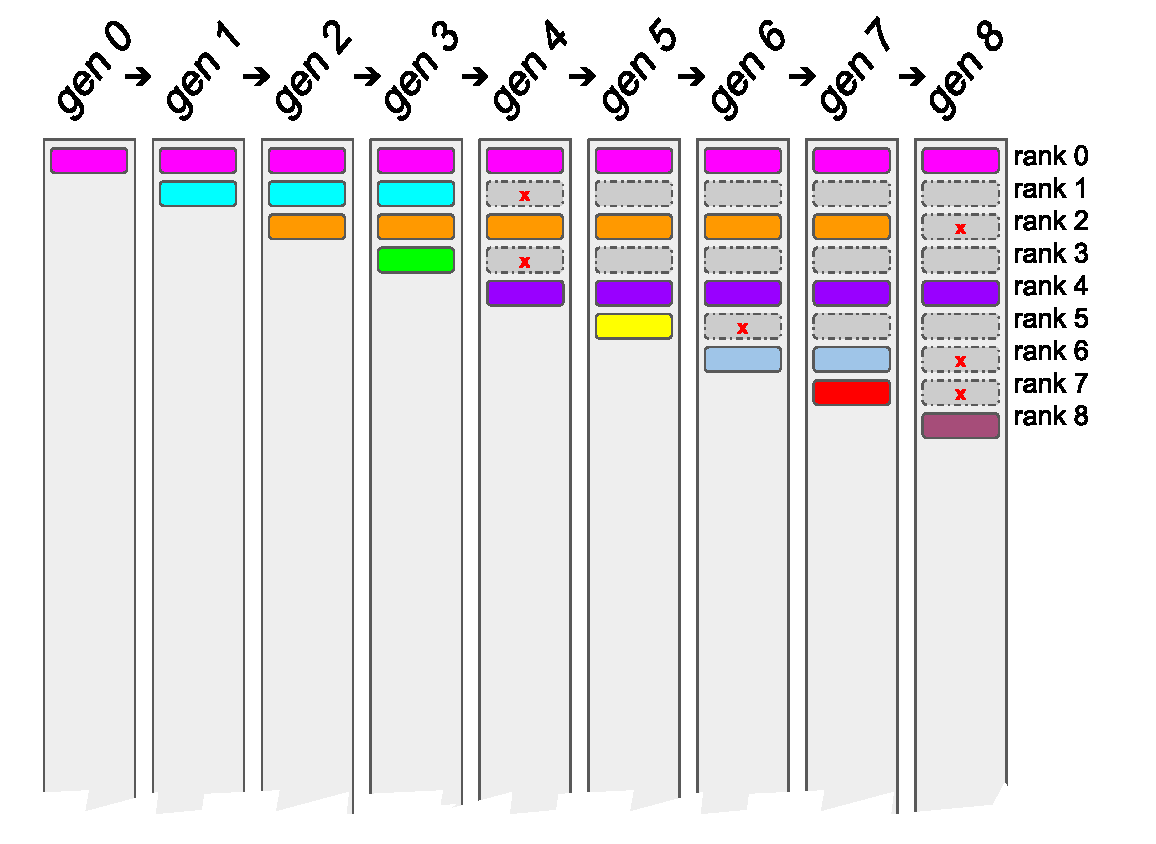
\includegraphics[width=\textwidth]{img/deposit-prune-example}
  \caption{
    Working principle of hereditary stratigraphy.
    Each generation, hereditary stratigraph genome annotations are inherited and a new randomly-generated ``fingerprint'' differentia is appended.
    Hereditary stratigraph annotations are depicted as tall squared boxes with differentia, depicted as squat rounded boxes, nested within.
    Differentia color represents randomly-generated differentia value.
    Comparison of aligned differentia reveals time of ancestral divergence (i.e., mismatching differentia).
    Differentia may be ``pruned'' to save space (shown in the diagram as a red $x$).
    However, this space savings comes at a trade-off of inference resolution.
    Figure \ref{fig:retention-policy-matrix} overviews strategies for differentia pruning and their corresponding space-resolution trade-offs.
  }
  \label{fig:deposit-prune-example}
\end{figure}
